% This template was created by Chris Hoofnagle for 
% the Berkeley Center for Law & Technology. If you 
% work for UCB, you are welcome to use it.


\documentclass[letterpaper,12pt,openbib]{report}

% This is a "report" document class, which means that it has chapters
% and formatting like a book, but fundamentally is a design for
% one-sided printing. There are many options to change the underlying
% design---you can change the font, paper size, etc with these 
% options below. Just put the options in the braces of 
% \documentclass

% Documentclass: Report Options: a4paper, a5paper, b5paper, letterpaper, legalpaper, landscape, 11pt, 12pt, twoside, twocolumn, notitlepage, openright, draft, fleqn, leqno, openbib

%\usepackage[utf8]{inputenc}
\usepackage{graphicx}
\usepackage{lipsum} % generates lorem ipsum filler text
\usepackage[most,many,skins,breakable]{tcolorbox}
\usepackage{xcolor}
\usepackage{tikz}
\usepackage{tikzpagenodes}
\tcbuselibrary{skins,breakable,xparse}
\usepackage{fancyhdr}
\usepackage[default,scale=0.95]{opensans}
\usepackage[hidelinks]{hyperref} % the hidelinks option prevents those terrible boxes from appearing in your print pdf
\usepackage[backend=biber,language=american,style=verbose]{biblatex}
\addbibresource{bibliography.bib}
\usepackage[headheight=15pt,hmarginratio=1:1]{geometry}

%%%%%%%%%%%%%%%%%%%%%%%%
%
% Berkeley Colors - Global (changing these will alter the whole
% document)
%
%%%%%%%%%%%%%%%%%%%%%%%%

% Deep blue and gold
\definecolor{berkeleyblue}{HTML}{C33531}
\definecolor{berkeleygold}{HTML}{A0C8EB}
% Light blue and gold
\definecolor{founderblue}{HTML}{C33531}
\definecolor{founderyellow}{HTML}{C4820E}

%%%%%%%%%%%%%%%%%%%%%%%%
%
% Headings
%
%%%%%%%%%%%%%%%%%%%%%%%%

\fancyhf{}
% If you'd like, you can put the title of the report in the header
% Just erase title of report if not

\small\fancyhead[R] {\color{founderblue}The Coding Industry:  A technological retrospective and forecast. ~ \thepage}
% This adds the line below the header. You can make it thicker or thinner by editing the 0.4 value
\renewcommand{\headrulewidth}{0.4pt}
% This template only uses a header because a document with footnotes
% looks strange with a footer. But if you want a footer, just 
% uncomment the lines below
%\small\fancyfoot[R] {\color{founderblue}Title of Report ~ \thepage}
%\renewcommand{\footrulewidth}{0.0pt}

%%%%%%%%%%%%%%%%%%%%%%%%
%
% Customizing Fonts & Title Formats - Global
%
%%%%%%%%%%%%%%%%%%%%%%%%

% This section specifies the fonts and their sizes and 
% colors for the headings. Notice that the package gives
% you serif headings and san serif body text.

\usepackage{titlesec}
\usepackage{fontspec}

% The headings are Berkeley's Old Style Fonts!
% I don't like the new fonts, which are licensed from
% Adobe --- why would you do that?

\newfontfamily\headingfont{UCBerkeleyOS.otf}[
BoldFont = UCBerkeleyOSBold.otf,
ItalicFont = UCBerkeleyOSItalic.otf,
BoldItalicFont = UCBerkeleyOSBoldItalic.otf]

% This controls the chapter headings

\titleformat{\chapter}{\fontsize{30}{60}\headingfont}{\color{founderblue}\thechapter\fontsize{90}{60}}{10pt}{\thispagestyle{empty}\color{founderblue}\Huge\bfseries}

% This controls the section and subsection headings in the chapters
% Notice that the headings in the chapter are numbered, e.g.
% 1.1 A Lesson in Latin. If you don't want section numbering,
% remove \thesection and/or \thesubsection

\titleformat{\section}{\Large\headingfont}{}{0pt}{\color{founderblue}{\thesection} \ }[{\titlerule[0.8pt]}]

\titleformat{\subsection}{\large\headingfont}{}{0pt}{\color{founderblue}{\thesubsection} \ }[{\titlerule[0.8pt]}]

% This customizes the sections in the executive summary so that they
% will not be numbered.

\titleformat{name=\section,numberless}
{\Large\headingfont}{}{-4pt}{\color{founderblue} \ }[{\titlerule[0.8pt]}]

\titleformat{name=\subsection,numberless}
{\large\headingfont}{}{-4pt}{\color{founderblue} \ }[{\titlerule[0.8pt]}]

%%%%%%%%%%%%%%%%%%%%%%%%
%
% Sidebar Environment: mdframed
%
%%%%%%%%%%%%%%%%%%%%%%%

\usepackage{amstext}
\usepackage{mathtools}
\usepackage[framemethod=TikZ]{mdframed}


\mdfdefinestyle{custom}{frametitle={\colorbox{berkeleygold}{\space You must specify a title for your box \space}},
     frametitlefont=\textbf,
     backgroundcolor=founderblue!20,
     linecolor=founderblue!70,
     innertopmargin=10pt,
     frametitleaboveskip=-\ht\strutbox,
     skipabove=\topskip,
     skipbelow=\topskip}




%\newenvironment{sidebar}[1]
% \mdfsetup{%
% % Replace berkeleygold with white if you'd like
%     frametitle={\colorbox{berkeleygold}{\space#1\space}},
%     frametitlefont=\textbf,
%     backgroundcolor=founderblue!20,
%     linecolor=founderblue!70,
%     innertopmargin=10pt,
%     frametitleaboveskip=-\ht\strutbox,
% %    frametitlealignment=\left,
%     skipabove=\topskip,
%     skipbelow=\topskip
%     }%
%   \begin{mdframed}%
%   }
%   {\end{mdframed}}

%%%%%%%%%%%%%%%%%%%%%%%%
%
% Sidebars with tcolorbox -- Mybox
%
%%%%%%%%%%%%%%%%%%%%%%%

\newtcolorbox{mybox}[2][]{enhanced, interior hidden, 
coltitle=black, fonttitle=\bfseries\headingfont\large,
attach boxed title to top left={yshift=-2.5mm},
boxed title style={empty, size=small, top=1mm, bottom=2pt},
%boxed title=0.5\linewidth,
frame code={
\path (title.east|-frame.north) coordinate (aux);
\path[draw=founderblue, fill=founderblue!20, line width=0.5mm, rounded corners]
(frame.west) |- ([xshift=-2.5mm]title.north east) to[out=0, in=180] ([xshift=7.5mm]aux)-|(frame.east)|-(frame.south)-|cycle;  
},
title={#2},#1}

%%%%%%%%%%%%%%%%%%%%%%%%
%
% General Guidance
%
%%%%%%%%%%%%%%%%%%%%%%%

%\flushbottom

%The \flushbottom declaration makes all text pages the same height, adding extra vertical space when necessary to fill out the page.

%\onecolumn
%The \onecolumn declaration starts a new page and produces single-column output.

%\raggedbottom
%The \raggedbottom declaration makes all pages the height of the text on that page. No extra vertical space is added.

%\twocolumn
%The \twocolumn declaration starts a new page and produces two-column output.

%%%%%%%%%%%%%%%%%%%%%%%%
%
% Document Content Starts Here
%
%%%%%%%%%%%%%%%%%%%%%%%


\title{Put title here, and in the title.tex file}

\begin{document}

% The title page appearance is controlled by a separate file named titlepage.tex
\begin{titlepage}
\pagecolor{founderblue}
       \vspace*{1cm}


% This controls the title
% You can reposition this element by editing the numeric
% values in \node (1,1). The first value controls the 
% horizontal placement, the second the vertical.

\tikz[overlay, remember picture] \node at (1,1) {
\begin{tcolorbox}[colback=berkeleygold,width=15cm,halign=right,boxrule=0pt]%%
\headingfont{\fontsize{40}{60}\selectfont The Coding Industry: }

\end{tcolorbox}
};

% This controls the subtitle
\tikz[overlay, remember picture] \node at (1,-1.4) {
\begin{tcolorbox}[colback=berkeleygold,width=15cm,halign=right,boxrule=0pt]%%
\headingfont{\fontsize{30}{60}\selectfont A technological retrospective and technological forecast.}

\end{tcolorbox}
};

% This places the front cover logo. Replace logo.png with
% your logo
% You can reposition the logo by changing the node values
% 6.5 places the image in the center. The second number
% controls its vertical placement
\tikz[overlay, remember picture] \node at (6.5,-5) {
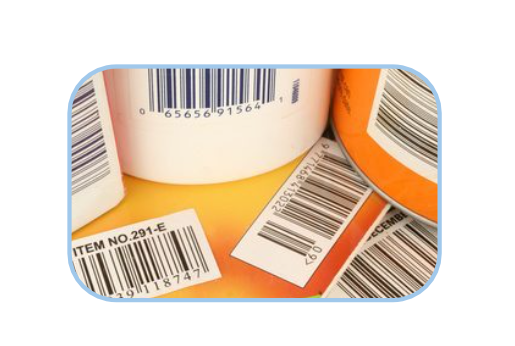
\includegraphics[width=0.7\textwidth]{logo.png}  


};

   

\vspace*{1cm}
% This controls the author block. You can add or reduce the
% number of authors by simply deleting text and the \\. Each
% \\ gives you a new line
\tikz[overlay, remember picture] \node at (-4,-8) {
\begin{tcolorbox}[colback=berkeleygold,width=15cm,halign=right,boxrule=0pt]%%
  \headingfont\Large Jerome A. Graves
\end{tcolorbox}
};
  
% This controls the date block. \today produces today's date.
% You can erase \today and replace it with something else
\tikz[overlay, remember picture] \node at (-4,-12) {
\begin{tcolorbox}[colback=berkeleygold,width=15cm,halign=right,boxrule=0pt]%%
  \headingfont\Large\today
\end{tcolorbox}


};
    



\end{titlepage}

% This makes the report have a white background
\pagecolor{white}

% Just comment out the next lines if you 
% do not want a table of contents

% This adds the Executive Summary to the TOC w/o a number
\addcontentsline{toc}{chapter}{Executive Summary}
\tableofcontents
% Note: to have a conclusion in the TOC without a number
% the addcontentsline command appears after \include conclusion
% below

% The content of the report is in subfiles that are
% imported below with the include command
% You can create more "chapters" by copying the chapter.tex
% files and using \include{chapterX} to include them in
% the report

\chapter*{Executive Summary}
\pagestyle{fancy}

Coding is an integral part of manufacturing. In every country in the world, there are strict rules for individual marking for products. Every product sold in a marketplace requires a barcode, even if you make it yourself. These can be \textbf{sell-by dates}, \textbf{UPC} or \textbf{EAN} numbers.


\bigskip
A  manufacturing company must have systems in place to individually mark items. These markings must have a level of visual fidelity to regional or international standards. And they should operate at a speed that doesnt slow doesnt production. As global demand has increased, the manufacturing industry has met the challenge with an increase in production (8.3percent in 2021). Marking technology has seen few improvements over the last 30 years and may soon become a bottleneck in production.

\bigskip
Most of the coding industry uses over-printers to complete coding, although conventional printing techniques are still used. Many commercially available manufacturing machines have hardpoint connections for the industry-leading coding printers. 

\bigskip
The main coding printing technologies are Dot Matrix, Inkjet, Laser and Thermal printers. Dot matrix creates codes that can be difficult to scan. Laser printers can only print conventionally and cannot over-print, making them unusable in many scenarios. Inkjet also has limitations in how it can be placed and used. Printing at steep angles or inverted is not possible. The introduction of wet ink also can cause havoc on a production line. Direct thermal requires thermal material to print on, usually thermal paper. This can cause issues as it needs to be transferred to the product, usually for a sticker label. These labels can be removed from products which is a less effective solution. 

\bigskip
By far the best and most used method of coding products is thermal transfer printing. Their printing method allows for the direct marking of many types of packaging materials, with high speeds and quality at an adorable price.

\bigskip
Although these printing machines have slightly different techniques, they all suffer from essentially the same limitations. 

\begin{itemize}
    \item Reliability/Durability
    \item High cost of consumables Ink, printheads
\end{itemize}

The mechanical nature of transferring ink to the material's surface means that these printers have many parts that can become worn over time, as well as physical limits to their achievable speed. As factory production speeds increase the prints per minute of the printerPPM increase and their consumable parts reach the end of their life much faster. This means partially stopping production by swapping the ink medium or a printhead.

\bigskip
Ink can also come in many forms but generally is shipped in small packets, where a large portion of the mass of the cartridge is plastic packaging. The most used technology currently (thermal transfer printing) has a 60-80percent ink transfer efficiency. These factors can have a significant effect on product margins. 

\bigskip
High-frequency UV laser marking is an advancing technology that addresses many of these issues. Laser making is a robust technology that has been used to mark packaging and products for over 30 years. It is an inkless technology that burns irremovable marks into the item. Its main limitation is that it can only be used on certain materials due to the high play nature of the laser?

\bigskip
UV lasers have less energy and work well on plastics. Also with High-frequency pulsing, there is greater control of the laser power, allowing for annealing effects on plastics. This inkless process doesn't require contact, reducing cost and dramatically increasing reliability. It is also faster than traditional printing with the slow machine being capable of 600/m/s, which is at the top end for overprinting. It is also far more accurate allowing for double the dpi (dots per inch) of a traditional over-printer. 




% The Asterix after chapter here excludes executive summary from the table of content and ensures it doesn't get a number (e.g. chapter 1)



%\section*{Introduction}
% The Asterix after section causes it to not be included in the table of contents

%\lipsum[1]

%\subsection*{Sub section title for exec summary}

%\lipsum[2-3]

\chapter{Introduction}
\pagestyle{fancy}

Coding machines are an integral part of the manufacturing industry and are an important part of how governments regulate products. The manufacturing industry grew by 8.3\% and is predicted to increase in the coming years.
As production output increases, overall production speeds will increase to meet the demand. This is directly proportional to the coding industry growth. Whether it be a sell-by date, barcode or an EAN number, products are legally required to be marked either in batches or individually. 

\bigskip
This job has traditionally been done by \textbf{over-printers}.


\bigskip

\section{What is an over-printer?}

Rather than a classic printer that feeds the material into its system, an over-printer is a machine designed to print directly on the material, from above (or other angles). The main benefit of this is the ability to mark products at different points with little interference in the assembly line.

\subsection{Intermittent and continuous printers?}

There are two main types of operation for over-printers, intermittent and continuous. They refer to the operation of the parent machine (the machine the printer is attached to). Some production lines operate in a stop-start fashion giving time to complete batch tasks before moving products to the next position. Other production lines work without stopping.

\begin{itemize}
    \item \textbf{Intermittent} printers are required if the production line stops and starts. They print on the substrate(material to be printed on) when it is stationary. They print on a flat surface with a mechanical arm in the printer that moves the printhead across the substrate.
    \item \textbf{Continuous} printers are used when the substrate does not stop. They print on the substrate as it is traveling. They usually print on a roller (see below). The substrate is moved by the parent machine (the machine the printer is attached to). The printing speed is also synchronized with the parent machine.
\end{itemize}

\subsection{Prints per minutes (PPM) Vs Print speed(mm/s)?}

A few values are used to show the speed of a printer. The most common are PPM and Print speed. The PPM is the maximum number of prints the machine can do in a minute. The print speed is the speed at which ink is transferred to the substrate. It is hard to draw any meaning from PPM  as manufacturers do not refer to the size of the printed image. Print speed better represents the printer's capability for high production as PPM can be calculated situationally.


\subsection{Left and right-hand printers?}

Most continuous over printers only print on the substrate in a given direction. Due to the variety of parent machines and the fact that cartridges need to be easy accesses, some companies produce mirror printers that operation the opposite direction.

\chapter{Current Technology}
\pagestyle{fancy}

There are two main over-printing technologies:

\begin{itemize}
    \item Thermal transfer
    \item Inkjet
  \end{itemize}

  \section{Inkjet}

  Inkjet printers use liquid ink in cartridges, and a  mechanical mechanism to move the nozzle across the substrate whiles the substrate is moved perpendicularly underneath. As such, Ink-jets are mostly continuous printers, although there are some intermittent variations.

  The main issue with ink-jets is the use of expensive liquid ink, which needs to be replaced often and can leak, causing massive production line issues. The quality can be mixed as time is needed for the ink to dry and smudging can occur. The level of smudging depends on the material printed on with less porous materials being worse. Also, printing must be done in a flat position, machines cant print inverted or at a steep angle. This creates limitations when installing the machines.


  \section{Thermal transfer}

  Thermal transfer printers use ink with wax on a roll of thin plastic ribbon. The machine unrolls this as ink is needed. To deposit the ink, the printhead presses the ribbon against the substrate and uses heater elements to melt and transfer the ink-wax mixture. 
  The printhead contains hundreds of heater elements in a horizontal line, each corresponding to a pixel of information.
  In intermittent printing, the printhead moves across the substrate using a mechanical mechanism activating different heater elements across the ribbon to transfer ink. 
  In continuous operation, the printhead synchronises its elements with the moving substrate underneath to deliver ink. This allows for print while inverted and at steep angles. There is very good ink adhesion with plastic materials. 
  
  \section{Hot Foil}

  Before thermal transfer in ink-jet, hot foil machines were the majority and they are still used today. The machine uses a similar process as a thermal transfer printer but uses a heated stamp instead of the elements. Every printed image used a different stamp configuration.

\chapter{Technological Limitations}
\pagestyle{fancy}

\section{Speed Limitations}
The speed limitation of an over-printer is determined by its mechanical design, the properties of the substrate and the ink used. The limitations with mechanical design can mostly be overcome without limit, but the chemical properties of currently available inks seem to be the industry's major limiting factor. 
There are over-printers that boast speeds of around 1m/s and a few special examples of even faster speeds of 1500m/s that require a particular substrate and ink combination, but in a future where production lines will have certain elements working  2-4m/s, the over-printer will become a bottleneck that can only be alleviated by buying multiple machines.

\section{Durability}
Over-printers have many mechanical elements. As production speed increases, over-printers will have to become larger and bulker.  The Mechanics that move the printhead at higher speeds will need to be more robust to counteract the momentum generated. They will use ink faster so they will need larger body sizes for ink storage.
Printheads can also be considered consumable they have a limited life and will need to be changed more often with increased production. Every time A printer ink needs to be changed the production line must stop (in that area).
These machines will reach a point where their size, cost and amount of human maintenance needed will make them an ineffective solution.

\section{Consumables}

As production speed increases so do the use of consumables. Most over-printer have warranties that require you to buy a particular brand of ink much like home printers. Unlike home printers, Industrial printers print continuously for up to 7 days a week. This generates a massive amount of usage that dwarfs the cost of the over-printer. An over-printer that is being used moderately can use £100,000 of ink in a year. As production speed increases, this cost will increase proportionally.
This cost is exacerbated by the fact that the machines don’t use 100% Ink in their cartridge. Depending on the style of the printer up to 50% of this will remain in the ink transmission medium depending on what is printed( thermal transfer printers).
Most inks are also sold on a transmission medium with a large amount of unrecyclable plastic, this also increases proportionally with production as well as shipping costs.








\chapter{Future Technologies}
\pagestyle{fancy}

\section{Laser markers and engravers}
Laser engraving/cutting and marking technology have been around for over 50 years. Generally, it is used on ceramics, wood and metals. They work by moving a high-powered laser over the surface of the substrate. The surface is burnt leaving an irremovable mark.

\section{Scanning lasers}
A scanning laser uses a set of small mirrors on rotating arms, known as a galvo, to direct its beam. Due to the mirrors' low mass, extremely fast movement can be attained. 

\section{High-frequency UV Laser Markers}
UV laser uses a different wavelength than standard laser markers and can be used on plastic materials. By modifying the pulse width and frequency, their burn effect can be minimised and instead activates annealing effects on the substrate, causing different contrast effects.

\section{Subtractive marking}
When dealing with thin, delicate materials etching the surface may cause excessive deformation. Subtractive marking is then used. The laser is configured to remove the ink from a darkened area on the packaging. All packaging is pre-printed with logos and general information externally before it reaches the production line. 
Adding a darkened square on each pack results in a minimal cost increase( If any), as the machines used in this printing process are more ink efficient.









%include{chapter5}
%include{conclusion}
% This adds the conclusion to the TOC without a number
%addcontentsline{toc}{chapter}{Conclusion}
% It is possible to add a bibliography here
\printbibliography
% This is the back cover
% The page background is Berkeley's dark blue color


\pagecolor{berkeleyblue}
\pagestyle{empty}

% This places the back cover logo. Replace logo.png with
% your logo
\tikz[overlay, remember picture] \node at (6.5,-14) {
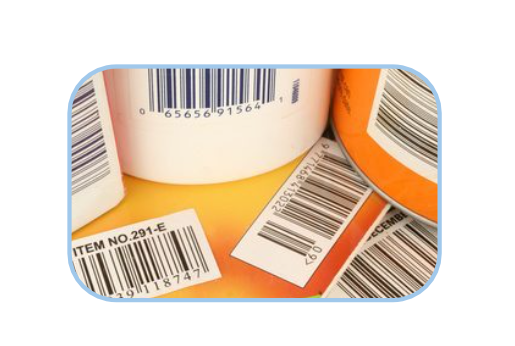
\includegraphics[width=0.7\textwidth]{logo.png}    
};

% This places those lines of text. Just erase Text 1, etc if you
% don't want any text

\tikz[overlay, remember picture] \node at (6.5,-17.7) {
\begin{tcolorbox}[colupper=white,colback=berkeleyblue,width=10cm,halign=left,boxrule=0pt]%%
  \headingfont\Large 
Jerome A. Graves
\end{tcolorbox}
};



% This code creates decorative `colorboxes' for text
% illustrations and the like. Just uncomment it and place
% it in a chapter

% \begin{tcolorbox}[breakable,title={An example colorbox},
% colback=founderblue!5!white,
% colframe=founderblue!75!black,
% fonttitle=\headingfont\bfseries\large]
% Your text goes here.
% \tcbsubtitle[before skip=\baselineskip]%
% {You can also have subboxes}
% with extra content
% \tcbsubtitle[before skip=\baselineskip]%
% {Multiple rows}
% If you like it.
% \end{tcolorbox}


% This code creates a decorative text box. 
% Just uncomment it and place
% it in a chapter

% \begin{mybox}{Hello World!}

% This is the mybox environment.

% However, the problem with mybox is that they cannot break across pages :( So, they have to be pretty short. Otherwise use the colorbox

% \end{mybox}





\end{document}

